\documentclass[12pt,a4paper]{article}
\title{\textbf{Homework1}}
\author{Maedeh Karkhane Yousefi-98100991}
\usepackage{graphicx}
\usepackage{float}
\usepackage{amsmath}
\begin{document}
\maketitle
\textbf{1. Koch Curve}
\\For this coding of this exercise, two main functions on each vector is operated. At the beginning we have a list containing two points with arbitrary components. In every step the variable \textit{i} is set to \textit{1} and the operation happens while \textit{i} is not equal to the total number of points we have in the list. the first point that is inserted is the point that is transferred in the amount of 1/3 vector. the next point is first transferred in the amount of 2/3 vector and then rotates 60 degrees around the previous point. It's obvious that we need to have some kind of coordinated transition,too. 
 Overall three points are inserted between the head and tail of the previous vector, all of which are shown in the figure below.
\begin{figure}[hb]
	\centering
	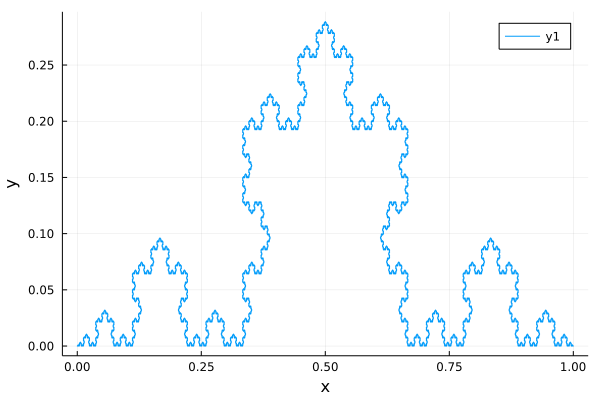
\includegraphics[width=0.5\textwidth]{Koch.png}
	\caption{Koch Curve is plotted for 10 steps. The initial points are:((0,0), (1,0))}
	\label{fig:mesh1}
\end{figure}


\textbf{2. Dragon Fractal}
\\our initial condition is two vectors that make a 90 degree angle with each other. The algorithm is just like the algorithm, used for Koch Curve. the main difference is that the rotation function one makes a 45 degree and once a -45 degree rotation.
\begin{figure}[H]
	\centering
	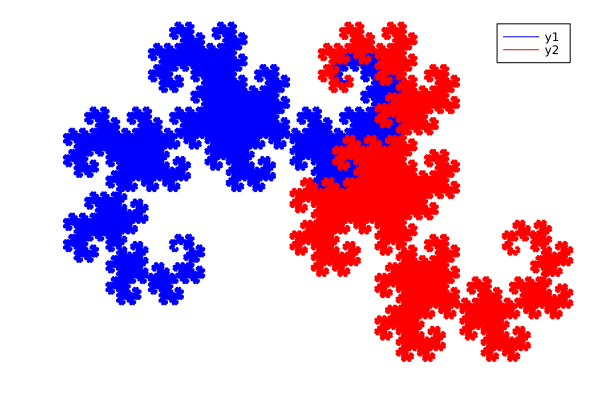
\includegraphics[width=0.5\textwidth]{DragonFractal.png}
	\caption{Dragon Fractal is plotted for 20 steps. The initial points were: ((0.00,0.00),(0.50, 0.49),(1.00,0.00))}
	\label{fig:mesh2}
\end{figure}

There is another result I ran into while coding this exercise, which I looked it up in the internet and found out it is named \textbf{Levy Dragon}, which is really beautiful actually!
\begin{figure}[H]
	\centering
	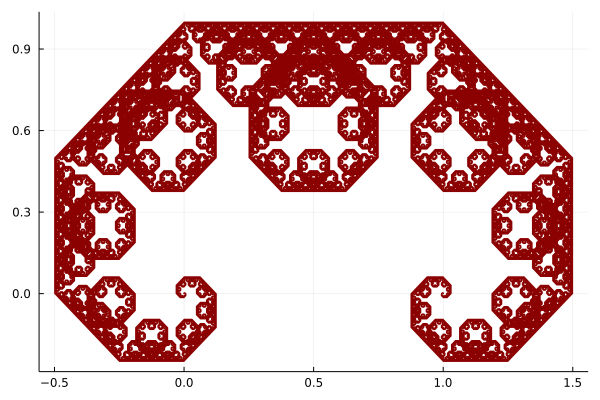
\includegraphics[width=0.5\textwidth]{Levy_dragon.png}
	\caption{Levy Dragon}
	\label{fig:mesh3}
\end{figure}


\textbf{3. Sierpinski Triangle}
\\In this code I stored the final triangles that are produced at the end of the process in separated lists, all in one \textit{$resutl_triangles$} list. For each triangle in the \textbf{$result_triangles$}, we make three empty lists representing the three triangles that produce per triangle. the first innermost \textit{for loop} goes through each point of the particular triangle to scale the points, creating the first new triangle and pushes the components of the vertices into the \textit{$first_triangle$}.
the second innermost \textit{for loop} pushes the components of the second and third new triangles that are in fact the transferred vertices of the first new triangle. Eventually the \textbf{$result_triangles$} becomes the  \textit{newOnes}, which consists of these three new triangles.
what I thought at first was that I need \textbf{all} the triangles made along the process, which was not the case at all!
\\At last I built a loop over each triangle to plot this figure below.
\begin{figure}[H]
	\centering
	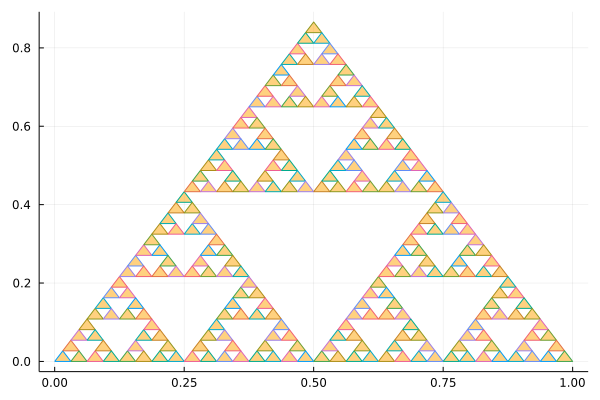
\includegraphics[width=0.5\textwidth]{SierpinskiTriangle.png}
	\caption{Sierpinski triangle is plotted for 5 steps.The main triangle's vercies are: ((0.0,0.0), (0.5,sqrt(3)/2),(1.0,0.0],[0.0,0.0))}
	\label{fig:mesh4}
\end{figure}


\textbf{4. Khayyam Triangle}
\\For this code I intended to store all the khayyam numbers in a list named \textbf{numberslist}. So, basically I added the first two elements of this series myself, and started the loop for creating the numbers from step 3. I set a condition that the first and the last element of each  series of numbers in each step, is \textit{1} and new numbers are created as shown bellow:
\[number_{R,n}=number_{R-1,n-1} + number{R-1, n}\]
consider R as each row of elements in the Khayyam triangle, and n as the number of each element in one row.
\\At the end all of these numbers are pushed into a list named \textit{R} containing the fist and last number \textit{1}. All of these \textit{R}s are pushed into the main list. 
\\for plotting, if we consider the starting point at (x,y)=(0.0, 0.0), we can observe a pattern in the sequence of the elements' positions, such that each row decrease by one {\textit{y-=1}) and each element in that row increase by one(\textit{x+=1/2}), taking note of the fact that the x component of the first element of each row is the row's number multiplied by 1/2. 
\\In the loop it will be check whether the number is even or not, and then it's position pushed into even or odd number's poses' list,respectively to be drawn with particular colors. 
\begin{figure}[H]
	\centering
	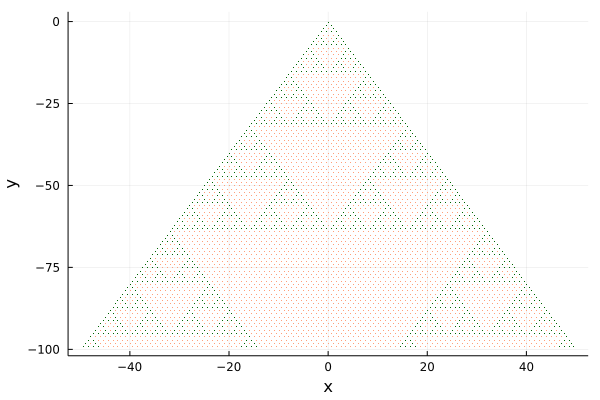
\includegraphics[width=0.5\textwidth]{KhayyamTriangle.png}
	\caption{Khayyam triangle is plotted for 100 steps. The starting point is at (0.0, 0.0).}
	\label{fig:mesh5}
\end{figure}

\textbf{5. Random Sierpinski Triangle}
\\In this random version of Sierpinski Triangle, I considered 3 functions, that scale the point and transfer it to two different directions. the point is randomly built and putted randomly into one of these functions. this process is repeated for each point several times and the final point is pushed into the \textit{finalPoints} list. we run the code for enough number of points till the Sierpinski Triangle is observed. 
\begin{figure}[H]
	\centering
	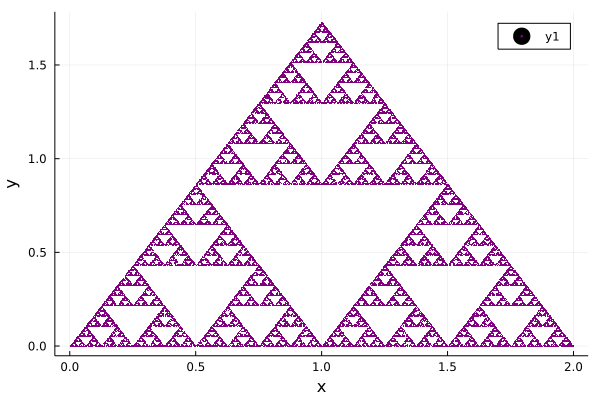
\includegraphics[width=0.5\textwidth]{SierpinskiRandomTriangle.png}
	\caption{Random Sierpinski triangle is plotted for 50000 points and repeated 100 times for each point.}
	\label{fig:mesh6}
\end{figure}


\textbf{6. Random Barnsley Fern}
\\By measuring and the information available in internet, accurate transfer and rotational matrices were built and introduced as four functions. assuming the starting point have the components (0.0,0.0) and putting other random points randomly into one of these four functions can lead us to the desired figure. Of course we must take into account that the probability of choosing these functions randomly is different from one another; Otherwise, the Barnsley Fern is going to be imperfect! Therefore, I used the \textit{StatsBase} package in julia to include this weight characteristic. 
the functions are:
\\f1=
$\begin{bmatrix}
0 & 0\\
0 & 16
\end{bmatrix}
\begin{bmatrix}
x\\
y
\end{bmatrix}$

f2=
$\begin{bmatrix}
0.85 & 0.04\\
-0.04 & 0.85
\end{bmatrix}
\begin{bmatrix}
x\\
y
\end{bmatrix}
+\begin{bmatrix}
0\\
1.6
\end{bmatrix}$

f3=
$\begin{bmatrix}
0.2 & -0.26\\
0.23 & 0.22
\end{bmatrix}
\begin{bmatrix}
x\\
y
\end{bmatrix}
+\begin{bmatrix}
0\\
1.6
\end{bmatrix}$

f4=
$\begin{bmatrix}
-0.15 & 0.28\\
0.26 & 0.24
\end{bmatrix}
\begin{bmatrix}
x\\
y
\end{bmatrix}
+\begin{bmatrix}
0\\
0.44
\end{bmatrix}$
\\All of these functions are chosen 1\%, 85\%, 7\% and 7\% of the time, sequentially.
\begin{figure}[H]
	\centering
	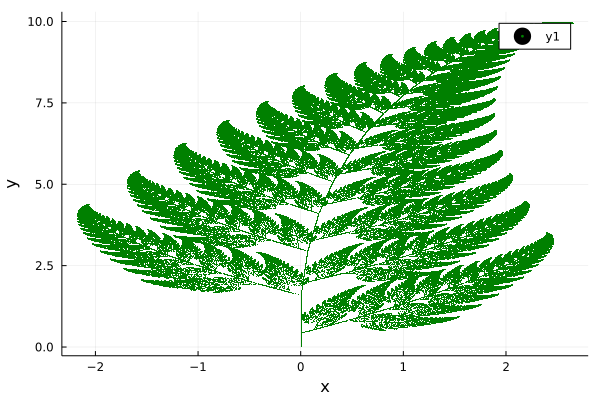
\includegraphics[width=0.5\textwidth]{RandomBarnsleyFern.png}
	\caption{Random Barnsley Fern is plotted for 500000 points and repeated 100 times for each point.The first point has components (0.0, 0.0)}
	\label{fig:mesh7}
\end{figure}
\end{document}
